\documentclass[11pt,a4paper]{article}
\usepackage{mathpazo}
\usepackage{verbatim}
\usepackage{bm}
\usepackage{tikz}
\usetikzlibrary{intersections,calc,through,arrows.meta,shapes.geometric}
\tikzset {>=Stealth}

\usepackage{url}

\newtheorem{theorem}{Theorem}
\newtheorem{definition}{Definition}

\textwidth=15cm
\textheight=23cm
\topmargin=0pt
\headheight=0pt
\oddsidemargin=2em
\headsep=0pt
\parindent=0pt
\renewcommand{\baselinestretch}{1.15}
\setlength{\parskip}{0.3\baselineskip plus 1pt minus 1pt}

\newcommand*{\qed}{\hfill\rule{1ex}{1.5ex}}

\newenvironment{form}[1]{%
\begin{displaymath}%
\renewcommand{\arraystretch}{#1}%
\begin{array}{lcl}}%
{\end{array}%
\end{displaymath}%
}

\begin{document}

\thispagestyle{empty}
\begin{center}
\textbf{\LARGE The Five-Color Theorem}

\bigskip

\textbf{\Large Moti Ben-Ari\\\bigskip\url{http://www.weizmann.ac.il/sci-tea/benari/}}

Version 1.0
\end{center}

\begin{footnotesize}
\begin{center}
\copyright{}\  2021 by Moti Ben-Ari. 
\end{center}
This work is licensed under the Creative Commons Attribution-ShareAlike 3.0 Unported License. To view a copy of this license, visit \url{http://creativecommons.org/licenses/by-sa/3.0/} or send a letter to Creative Commons, 444 Castro Street, Suite 900, Mountain View, California, 94041, USA.
\end{footnotesize}

\section{Planar maps and graphs}\label{s.planar}

\begin{theorem}
A planar map can be colored with four colors so that no adjacent regions share the same color.
\end{theorem}

The proof of this theorem is extremely difficult; here we prove the much simpler five-color theorem, originally proved in the nineteenth century.

\begin{theorem}
A planar map can be colored with five colors so that no adjacent regions share the same color.
\end{theorem}

\begin{definition}
A \textit{planar map} is a set of regions in the plane sharing boundaries. A \textit{coloring} of a map is an assignment of a color to each region such that regions sharing a boundary are assigned different colors.\footnote{Regions not sharing a boundary may be considered as ``the same,'' for example, state of Alaska and the state of Washington both belong to the United States, although they do not share a boundary and it is impossible to drive from one state to the other without passing through a different country (Canada).}
\end{definition}

The following diagrams show a planar map with ten regions. The left diagram shows a five-coloring and the right diagram shows a four-coloring.

\begin{center}
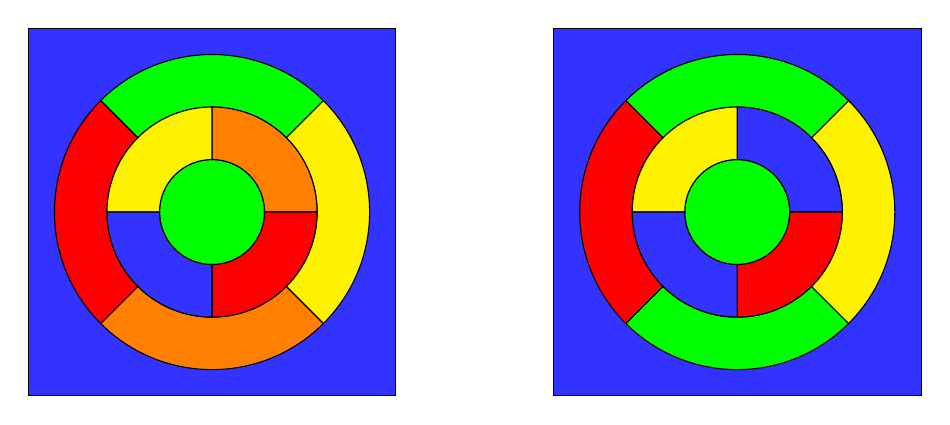
\begin{tikzpicture}[scale=.667]
\draw[fill=blue!80] (-3.5,-3.5) rectangle +(7,7);

\draw[fill=green] (0:1) 
  arc [start angle=0,  end angle=360, radius=1];

\draw[fill=green] (45:2) --
      (45:3)  arc[start angle=45,  end angle=135, radius=3] --
      (135:2) arc[start angle=135, end angle=45,  radius=2];
\draw[fill=orange] (-45:2) --
      (-45:3)  arc[start angle=-45,  end angle=-135, radius=3] --
      (-135:2) arc[start angle=-135, end angle=-45,  radius=2];
\draw[fill=yellow] (45:2) --
      (45:3)  arc[start angle=45,  end angle=-45, radius=3] --
      (-45:2) arc[start angle=-45, end angle=45,  radius=2];
\draw[fill=red] (135:2) --
      (135:3)  arc[start angle=135,  end angle=225, radius=3] --
      (225:2) arc[start angle=225, end angle=135,  radius=2];

\draw[fill=orange] (0:1) --
      (0:2)  arc[start angle=0,  end angle=90, radius=2] --
      (90:1) arc[start angle=90, end angle=0,  radius=1];
\draw[fill=red] (0:1) --
      (0:2)  arc[start angle=0,  end angle=-90, radius=2] --
      (-90:1) arc[start angle=-90, end angle=0,  radius=1];
\draw[fill=yellow] (90:1) --
      (90:2)  arc[start angle=90,  end angle=180, radius=2] --
      (180:1) arc[start angle=180, end angle=90,  radius=1];
\draw[fill=blue!80] (180:1) --
      (180:2)  arc[start angle=180,  end angle=270, radius=2] --
      (270:1) arc[start angle=270, end angle=180,  radius=1];

\begin{scope}[xshift=10cm]
\draw[fill=blue!80] (-3.5,-3.5) rectangle +(7,7);

\draw[fill=green] (0:1) 
  arc [start angle=0,  end angle=360, radius=1];

\draw[fill=green] (45:2) --
      (45:3)  arc[start angle=45,  end angle=135, radius=3] --
      (135:2) arc[start angle=135, end angle=45,  radius=2];
\draw[fill=green] (-45:2) --
      (-45:3)  arc[start angle=-45,  end angle=-135, radius=3] --
      (-135:2) arc[start angle=-135, end angle=-45,  radius=2];
\draw[fill=yellow] (45:2) --
      (45:3)  arc[start angle=45,  end angle=-45, radius=3] --
      (-45:2) arc[start angle=-45, end angle=45,  radius=2];
\draw[fill=red] (135:2) --
      (135:3)  arc[start angle=135,  end angle=225, radius=3] --
      (225:2) arc[start angle=225, end angle=135,  radius=2];

\draw[fill=blue!80] (0:1) --
      (0:2)  arc[start angle=0,  end angle=90, radius=2] --
      (90:1) arc[start angle=90, end angle=0,  radius=1];
\draw[fill=red] (0:1) --
      (0:2)  arc[start angle=0,  end angle=-90, radius=2] --
      (-90:1) arc[start angle=-90, end angle=0,  radius=1];
\draw[fill=yellow] (90:1) --
      (90:2)  arc[start angle=90,  end angle=180, radius=2] --
      (180:1) arc[start angle=180, end angle=90,  radius=1];
\draw[fill=blue!80] (180:1) --
      (180:2)  arc[start angle=180,  end angle=270, radius=2] --
      (270:1) arc[start angle=270, end angle=180,  radius=1];
\end{scope}
\end{tikzpicture}
\end{center}

\begin{definition}
A \emph{graph} is a set of \emph{vertices} $V$ and a set of \emph{edges} $E$, such that each edge is incident with exactly two vertices.

A \emph{planar graph} is a graph such that no edges cross each other. In a planar graph, areas enclosed by a set of edges are called \emph{faces}.

A \emph{coloring} of a planar graph is an assignment of colors to vertices such that no two vertices of the same color are connected by an edge.
\end{definition}

Planar maps and planar graphs are dual and it is convenient to treat coloring problems in graphs rather than maps.

\begin{theorem}
Given a planar map, a planar graph can be constructed such for each coloring of the regions of the map, there is a coloring of the vertices of the graph, and conversely.
\end{theorem}

\textbf{Proof}
Construct one vertex for each region and construct an edge between two vertices iff the regions are share a boundary.\qed

The following diagram shows how a planar graph can be constructed and colored based on the planar map shown above.

\begin{center}
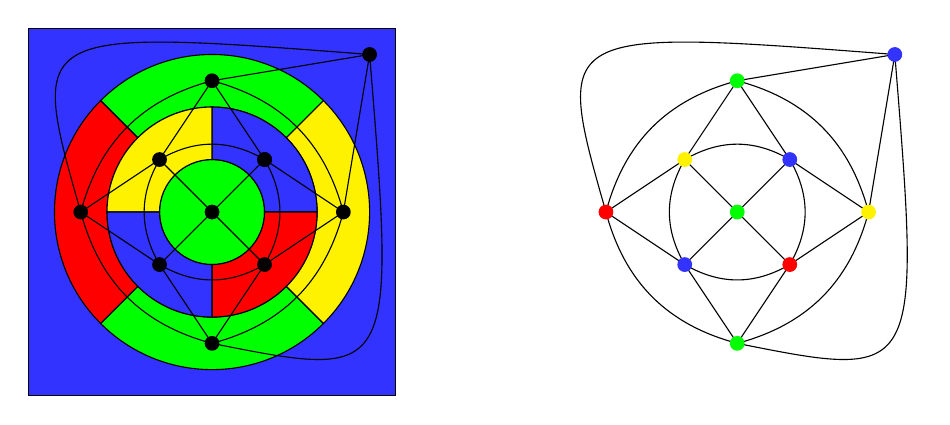
\begin{tikzpicture}[scale=.667]

\draw[fill=blue!80] (-3.5,-3.5) rectangle +(7,7);

\draw[fill=green] (0:1) 
  arc [start angle=0,  end angle=360, radius=1];

\draw[fill=green] (45:2) --
      (45:3)  arc[start angle=45,  end angle=135, radius=3] --
      (135:2) arc[start angle=135, end angle=45,  radius=2];
\draw[fill=green] (-45:2) --
      (-45:3)  arc[start angle=-45,  end angle=-135, radius=3] --
      (-135:2) arc[start angle=-135, end angle=-45,  radius=2];
\draw[fill=yellow] (45:2) --
      (45:3)  arc[start angle=45,  end angle=-45, radius=3] --
      (-45:2) arc[start angle=-45, end angle=45,  radius=2];
\draw[fill=red] (135:2) --
      (135:3)  arc[start angle=135,  end angle=225, radius=3] --
      (225:2) arc[start angle=225, end angle=135,  radius=2];

\draw[fill=blue!80] (0:1) --
      (0:2)  arc[start angle=0,  end angle=90, radius=2] --
      (90:1) arc[start angle=90, end angle=0,  radius=1];
\draw[fill=red] (0:1) --
      (0:2)  arc[start angle=0,  end angle=-90, radius=2] --
      (-90:1) arc[start angle=-90, end angle=0,  radius=1];
\draw[fill=yellow] (90:1) --
      (90:2)  arc[start angle=90,  end angle=180, radius=2] --
      (180:1) arc[start angle=180, end angle=90,  radius=1];
\draw[fill=blue!80] (180:1) --
      (180:2)  arc[start angle=180,  end angle=270, radius=2] --
      (270:1) arc[start angle=270, end angle=180,  radius=1];


\foreach \x/\y/\name in {
    0/0/O,
    3/3/Z,
    1/1/E,-1/1/F,-1/-1/G,1/-1/H,
    0/2.5/A,2.5/0/B,0/-2.5/C,-2.5/0/D,
    } {
  \fill (\x,\y) coordinate(\name) circle(4pt);
}

\draw (E) -- (O) -- (F);
\draw (G) -- (O) -- (H);
\draw (E) to [bend right=30] (F) to [bend right=30] (G) 
          to [bend right=30] (H) to [bend right=30] (E);
\draw (A) -- (E) -- (B) -- (H) -- (C) -- (G) -- (D) -- (F);
\draw (A) to [bend right=30] (D) to [bend right=30] (C) 
          to [bend right=30] (B) to [bend right=30] (A);

\draw (F) -- (A) -- (Z) -- (B);
\draw (C) .. controls (3.5,-3.2) .. (Z);
\draw (D) .. controls (-3.5,3.5) .. (Z);

\begin{scope}[xshift=10cm]

\foreach \x/\y/\name in {
    0/0/O,
    3/3/Z,
    1/1/E,-1/1/F,-1/-1/G,1/-1/H,
    0/2.5/A,2.5/0/B,0/-2.5/C,-2.5/0/D,
    } {
  \coordinate(\name) at (\x,\y);
}

\draw (E) -- (O) -- (F);
\draw (G) -- (O) -- (H);
\draw (E) to [bend right=30] (F) to [bend right=30] (G) 
          to [bend right=30] (H) to [bend right=30] (E);
\draw (A) -- (E) -- (B) -- (H) -- (C) -- (G) -- (D) -- (F);
\draw (A) to [bend right=30] (D) to [bend right=30] (C) 
          to [bend right=30] (B) to [bend right=30] (A);

\draw (F) -- (A) -- (Z) -- (B);
\draw (C) .. controls (3.5,-3.2) .. (Z);
\draw (D) .. controls (-3.5,3.5) .. (Z);

\foreach \cl/\x/\y in {
    green/0cm/0cm,
    blue!80/3cm/3cm,
    blue!80/1cm/1cm,
    yellow/-1cm/1cm,
    blue!80/-1cm/-1cm,
    red/1cm/-1cm,
    green/0cm/2.5cm,
    yellow/2.5cm/0cm,
    green/0cm/-2.5cm,
    red/-2.5cm/0cm
    }
  \fill[\cl] (\x,\y) circle (4pt);
\end{scope}

\end{tikzpicture}
\end{center}

We can further limit our graphs to those whose faces are \textit{triangular}.\footnote{The faces are not necessarily \textit{triangles} because the edges may be curved. By F\'{a}ry's theorem, any triangular planar graph can be be transformed to an equivalent graph with straight edges.}

The left diagram below shows that a square can be two-colored, but if it is triangulated (center), three colors are necessary. However, the goal is to prove that \emph{all} graphs can be five-colored, so if the triangulated graph is five-colored, so is the original graph, because deleting the extra edge does not invalidate the coloring (right).
\begin{center}
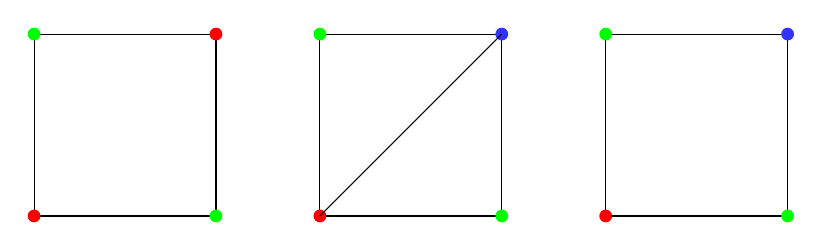
\begin{tikzpicture}[scale=.33]
\draw (-3.5,-3.5) rectangle +(7,7);
\fill[red] (-3.5,-3.5) circle(7pt);
\fill[green] (-3.5,3.5) circle(7pt);
\fill[green] (3.5,-3.5) circle(7pt);
\fill[red] (3.5,3.5) circle(7pt);
%\draw (-3.5,-3.5) -- (3.5,3.5);
\begin{scope}[xshift=11cm]
\draw (-3.5,-3.5) rectangle +(7,7);
\fill[red] (-3.5,-3.5) circle(7pt);
\fill[green] (-3.5,3.5) circle(7pt);
\fill[green] (3.5,-3.5) circle(7pt);
\fill[blue!80] (3.5,3.5) circle(7pt);
\draw (-3.5,-3.5) -- (3.5,3.5);
\end{scope}
\begin{scope}[xshift=22cm]
\draw (-3.5,-3.5) rectangle +(7,7);
\fill[red] (-3.5,-3.5) circle(7pt);
\fill[green] (-3.5,3.5) circle(7pt);
\fill[green] (3.5,-3.5) circle(7pt);
\fill[blue!80] (3.5,3.5) circle(7pt);
%\draw (-3.5,-3.5) -- (3.5,3.5);
\end{scope}
\end{tikzpicture}
\end{center}

\section{Euler's formula}

\begin{theorem}[Euler]\label{thm.euler}
Let $G$ be a connected planar graph with $V$ vertices, $E$ edges and $F$ faces. Then $V-E+F=2$.
\end{theorem}

\textbf{Proof} By induction on the number of edges. If the number of edges in the \emph{connected} graph is zero, there is only a single vertex and a single face, so $1-0+1=2$.

Let $G$ be a connected graph with $V$ vertices, $E$ edges and $F$ faces, and remove an edge $e$ connecting vertices $v_1,v_2$. There are two cases:

\textbf{Case 1} The graph becomes disconnected. Identify $v_1$ with $v_2$. The resulting graph $G'$ has fewer edges than $G$ so by the induction hypothesis, $(V-1)-(E-1)+F=2$ since the number of vertices is also reduced by one. Simplifying, we get $V-E+F=2$ for $G$.

\begin{center}
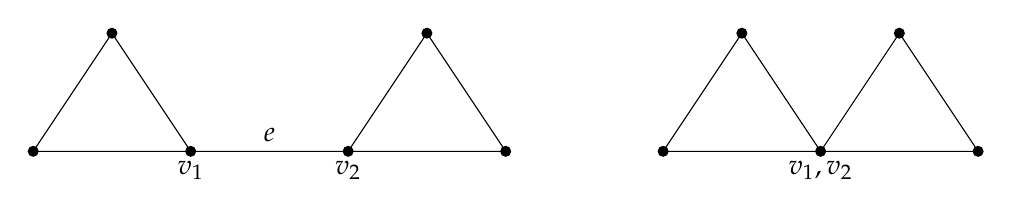
\begin{tikzpicture}
\foreach \x/\y in {0/0, 2/0, 1/1.5,4/0,6/0,5/1.5}
  \fill (\x,\y) circle (2pt);
\draw (2,0) -- (1,1.5) -- (0,0) -- (2,0) node[below] {$v_1$} -- node[above] {$e$} (4,0) node[below] {$v_2$} -- (6,0) -- (5,1.5) -- (4,0);
\begin{scope}[xshift=8cm]
\foreach \x/\y in {0/0, 2/0, 1/1.5,4/0,3/1.5}
  \fill (\x,\y) circle (2pt);
\draw (2,0) -- (1,1.5) -- (0,0) -- (2,0) node[below] {$v_1,v_2$} -- (4,0) -- (3,1.5) -- (2,0);
\end{scope}
\end{tikzpicture}
\end{center}

\textbf{Case 2} The graph remains connected. The resulting graph $G'$ has fewer edges than $G$ so by the induction hypothesis, $V-(E-1)+(F-1)=2$ since removing the edge joins two faces into one. Simplifying, we get $V-E+F=2$ for $G$.

\begin{center}
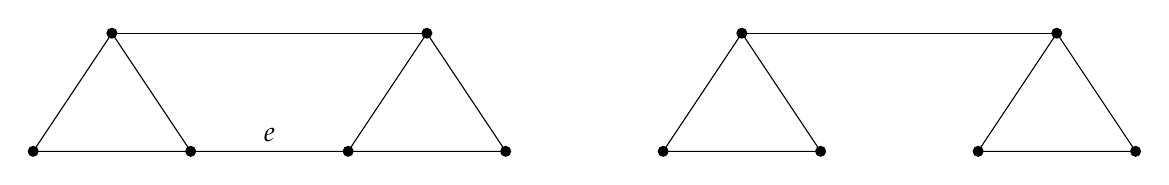
\begin{tikzpicture}
\foreach \x/\y in {0/0, 2/0, 1/1.5,4/0,6/0,5/1.5}
  \fill (\x,\y) circle (2pt);
\draw (2,0) -- (1,1.5) -- (0,0) -- (2,0) -- node[above] {$e$} (4,0) -- (6,0) -- (5,1.5) -- (4,0);
\draw (1,1.5) -- (5,1.5);
\begin{scope}[xshift=8cm]
\foreach \x/\y in {0/0, 2/0, 1/1.5,4/0,6/0,5/1.5}
  \fill (\x,\y) circle (2pt);
\draw (2,0) -- (1,1.5) -- (0,0) -- (2,0);
\draw (4,0) -- (5,1.5) -- (6,0) -- cycle;
\draw (1,1.5) -- (5,1.5);
\end{scope}
\end{tikzpicture}
\end{center}
\qed

\begin{theorem}
Let $G$ be a connected, triangulated planar graph. Then $E= 3V-6$.
\end{theorem}

For example, the planar graph in Section~\ref{s.planar} has $10$ vertices and $24= 3\cdot 10-6=24$ edges.

\textbf{Proof}
Each face is bounded by three edges, so $E=3F/2$ because each edge has been counted twice, once for each face it bounds. By Euler's formula:
\begin{form}{1}
E&=&V+F-2\\
E&=&V+2E/3-2\\
E&=&3V-6\,.
\end{form}
\vspace*{-5ex}
\qed

\newpage

\begin{theorem}\label{thm.count}
Let $G$ be a connected planar graph. Then $E\leq 3V-6$.
\end{theorem}

For the following graph, $E=8< 3\cdot 6 - 6= 12$.

\begin{center}
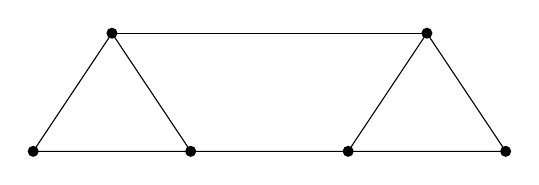
\begin{tikzpicture}
\foreach \x/\y in {0/0, 2/0, 1/1.5,4/0,6/0,5/1.5}
  \fill (\x,\y) circle (2pt);
\draw (2,0) -- (1,1.5) -- (0,0) -- (2,0) -- (4,0) -- (6,0) -- (5,1.5) -- (4,0);
\draw (1,1.5) -- (5,1.5);
\end{tikzpicture}
\end{center}

\textbf{Proof}
Triangulate $G$ to obtain $G'$. In $G'$, $E= 3V-6$ by Theorem~\ref{thm.count}. Now remove edges from $G'$ to obtain $G$. The number of vertices does not change so  $E\leq 3V-6$.
\qed

Here is the triangulated graph for which $E=12=3\cdot 6 - 6= 12$.
\begin{center}
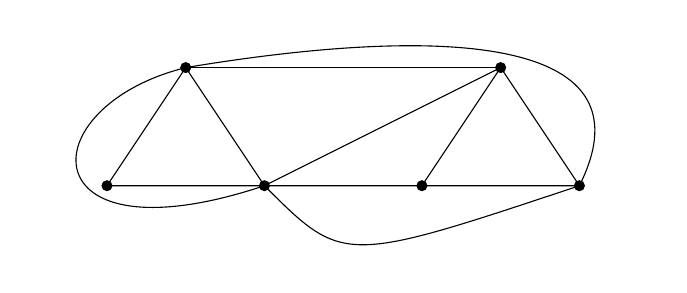
\begin{tikzpicture}
\foreach \x/\y in {0/0, 2/0, 1/1.5,4/0,6/0,5/1.5}
  \fill (\x,\y) circle (2pt);
\draw (2,0) -- (1,1.5) -- (0,0) -- (2,0) -- (4,0) -- (6,0) -- (5,1.5) -- (4,0);
\draw (1,1.5) -- (5,1.5);
\draw (2,0) -- (5,1.5);
\draw (2,0) .. controls (-1,-1) and (-1,1) .. (1,1.5);
\draw (2,0) .. controls (3,-1) .. (6,0) .. controls (7,2) and (4,2) .. (1,1.5);
\end{tikzpicture}
\end{center}

\section{Non-planar graphs}
Let us take a short detour to show how Theorems~\ref{thm.euler} and~\ref{thm.count} can be used to prove that certain graphs are not planar.

\begin{theorem}
$K_5$, the complete graph on five vertices, is not planar.
\end{theorem}

\begin{center}
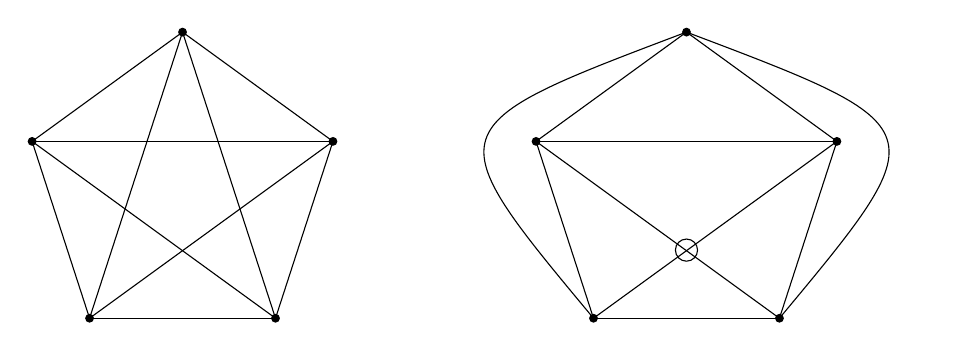
\begin{tikzpicture}[scale=.8]
\node (pentagon) [minimum size=4cm,regular polygon,regular polygon sides=5] at (0,0) {};
\draw (pentagon.corner 1) -- (pentagon.corner 2);
\draw (pentagon.corner 2) -- (pentagon.corner 3);
\draw (pentagon.corner 3) -- (pentagon.corner 4);
\draw (pentagon.corner 4) -- (pentagon.corner 5);
\draw (pentagon.corner 5) -- (pentagon.corner 1);
\draw (pentagon.corner 1) -- (pentagon.corner 3);
\draw (pentagon.corner 1) -- (pentagon.corner 4);
\draw (pentagon.corner 2) -- (pentagon.corner 4);
\draw (pentagon.corner 2) -- (pentagon.corner 5);
\draw (pentagon.corner 3) -- (pentagon.corner 5);

\foreach \corner in {1,2,3,4,5}
  \fill (pentagon.corner \corner) circle (2pt);

\begin{scope}[xshift=8cm]
\node (pentagon) [minimum size=4cm,regular polygon,regular polygon sides=5] at (0,0) {};
\draw (pentagon.corner 1) -- (pentagon.corner 2);
\draw (pentagon.corner 2) -- (pentagon.corner 3);
\draw (pentagon.corner 3) -- (pentagon.corner 4);
\draw (pentagon.corner 4) -- (pentagon.corner 5);
\draw (pentagon.corner 5) -- (pentagon.corner 1);
\draw (pentagon.corner 1) .. controls (-4,1) .. 
      (pentagon.corner 3);
\draw (pentagon.corner 1) .. controls (4,1) ..
      (pentagon.corner 4);
\draw (pentagon.corner 2) -- (pentagon.corner 4);
\draw (pentagon.corner 2) -- (pentagon.corner 5);
\draw (pentagon.corner 3) -- (pentagon.corner 5);

\foreach \corner in {1,2,3,4,5}
  \fill (pentagon.corner \corner) circle (2pt);
\draw (0,-.95) circle(5pt);
\end{scope}
\end{tikzpicture}
\end{center}
\textbf{Proof}
For $K_5$, $V=5$ and $E=10$. But $10 \not\leq 3\cdot 5 -6=9$.\qed

\newpage

\begin{theorem}
$K_{3,3}$, the bipartite graph with three vertices on each side, is not planar.
\end{theorem}

\begin{center}
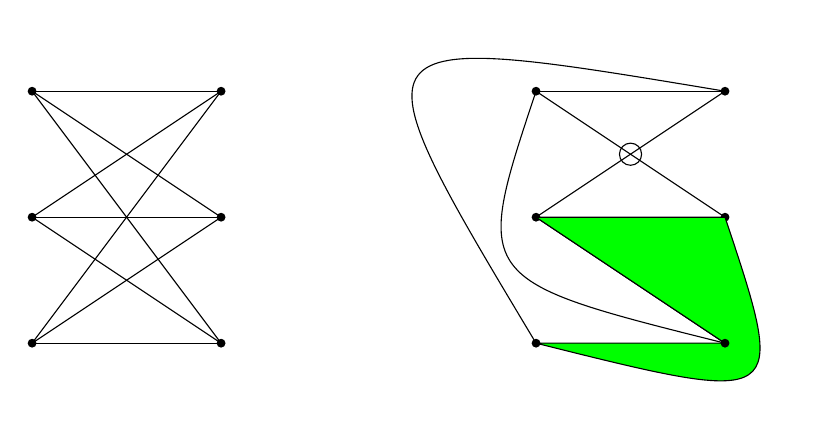
\begin{tikzpicture}[scale=.8]
\foreach \x/\y in {0/0,0/2,0/4,3/0,3/2,3/4}
  \fill (\x,\y) circle (2pt);
\draw (0,0) -- (3,0);
\draw (0,2) -- (3,2);
\draw (0,4) -- (3,4);
\draw (0,0) -- (3,2);
\draw (0,2) -- (3,4);
\draw (0,4) -- (3,0);
\draw (0,0) -- (3,4);
\draw (0,2) -- (3,0);
\draw (0,4) -- (3,2);
\begin{scope}[xshift=8cm]
\foreach \x/\y in {0/0,0/2,0/4,3/0,3/2,3/4}
  \fill (\x,\y) circle (2pt);
\draw (0,4) -- (3,4);
c\draw (0,2) -- (3,4);
\draw (0,4) .. controls (-1,1) .. (3,0);
\draw (0,0) .. controls (-3,5) .. (3,4);
\draw (0,2) -- (3,0);
\draw (0,4) -- (3,2);

\draw[fill=green] (0,0) -- (3,0) -- (3,0) -- (0,2)  -- (3,2) .. controls (4,-1) .. (0,0);
\fill (3,0) circle (2pt);
\draw (1.5,3) circle(5pt);
\end{scope}
\end{tikzpicture}
\end{center}
\textbf{Proof}
$V=6$ and $E=9$. By Theorem~\ref{thm.euler}, $F=E-V+2=9-6+2=5$. But each face is bounded by four edges, so $E=4F/2=10\neq 9$.\qed

\section{The degrees of the vertices}

\begin{definition}
$d(v)$, the degree of vertex $v$, is the number of edges incident with $v$.
\end{definition}
For the graph in Section~\ref{s.planar}, there are $8$ vertices in the two annuli, each of degree $5$; the vertices of the outer face and the inner circular face are each of degree $4$. Therefore:
\[
\sum_{v\in V} d(v) = 5\cdot 8 + 4\cdot 2=48\,.
\]
To get the total number of edges, divide by $2$ because  each edge was counted twice, once for each of the vertices it is incident to.

By generalizing the argument we get:
\begin{theorem}\label{thm.degrees}
Let $d_i, i=1,2,3,\ldots,k$ be the number of vertices of degree $i$ in a connected planar graph $G$ with $V$ vertices and $E$ edges, where $k$ is the highest degree of a vertex in $V$. Then:
\[
\sum_{v\in V} d(v) =\sum_{i=1}^{k} i\cdot d_i=2E\,.
\]
\end{theorem}

\begin{theorem}\label{thm.degree5}
Let $G$ be a connected planar graph with $E$ edges and $V$ vertices, and let $d_i,i=1,\ldots,k$ be the number of vertices of degree $i$, where $k$ is the highest degree of a vertex in $V$. Then there must be a vertex $v$ in $V$ such that $d(v) \leq 5$.
\end{theorem}
\textbf{Proof 1}
Clearly, if there are $d_1$ vertices of degree $1$, $d_2$ vertices of degree $2$, \ldots, $d_k$ vertices of degree $k$, then $V=\sum_{i=1}^{k}d_i$.  From Theorems~\ref{thm.count} and \ref{thm.degrees}:
\[
\sum_{i=1}^{k} i\cdot d_i=2E\leq 2(3V-6) = 6V-12=6\sum_{i=1}^{k} d_i -12\,.
\]
Therefore:
\[
\sum_{i=1}^{k} i\cdot d_i \leq 6\sum_{i=1}^{k} d_i -12\,,
\]
and:
\[
\sum_{i=1}^{k} (6-i)d_i> 12\,.
\]
Since $12>0$, for least one $i$, $6-i>0$ and for that $i$, $i<6$. \qed

\textbf{Proof 2} Let us compute the \emph{average} degree of the vertices, which is the sum of the degrees divided by the number of vertices:
\[
d_{\textit{\footnotesize avg}}=\frac{\sum_{i=1}^{k} i\cdot d_i}{V}\,.
\]
But the sum of the degrees is twice the number of edges which by Theorem~\ref{thm.count} gives:
\[
d_{\textit{\footnotesize avg}}=\frac{2E}{V}\leq \frac{6V-12}{V}=6-\frac{6}{V}<6\,.
\]
If the average degree is less than six, there must be a vertex of degree less than six.\qed


For the graph in Section~\ref{s.planar}, the sum of the degrees is $8\cdot 5 + 2\cdot 4=48$. There are $10$ vertices, so the average degree is $\frac{48}{10}=4.8$ and there must be a vertex of degree $4$ or less.

\section{The six-color theorem}

\begin{theorem}\label{thm.sixcolor}
Any planar graph $G$ can be six-colored.
\end{theorem}
\textbf{Proof} By induction on the number of vertices in $G$. The base case is any planar graph with six or fewer vertices, for which six colors clearly suffice.

For the inductive step, let $G$ be a planar graph. By Theorem~\ref{thm.degree5} it has a vertex $v$ with degree $5$ or fewer. Delete vertex $v$ to obtain $G'$. By the induction hypothesis, $G'$ can be six-colored, but $v$ has at most $5$ neighbors and at most $5$ colors are used to color them, so $v$ can be colored using the sixth color. \qed

\begin{center}
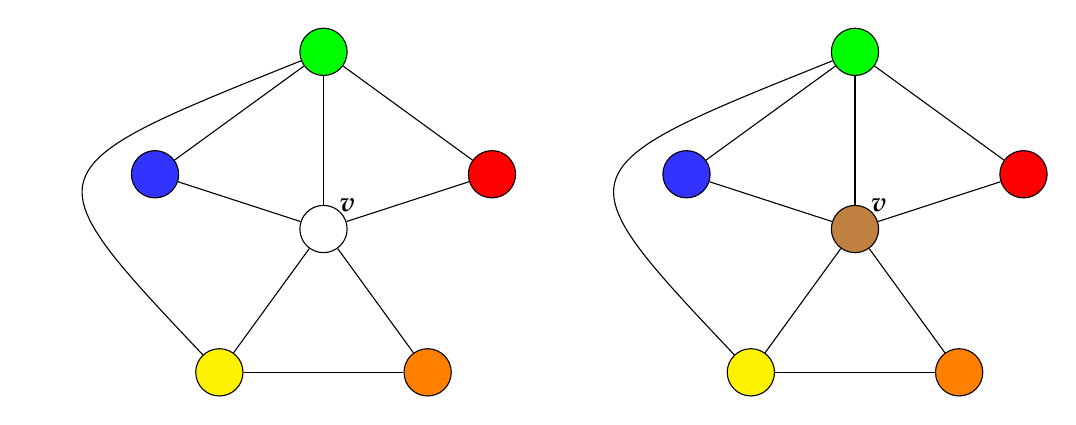
\begin{tikzpicture}[scale=.75,minimum size=6mm,inner sep=0pt]
\foreach \name/\color/\theta in
    {A/red/18,B/green/90,C/blue!80/162,D/yellow/234,E/orange/306}
  \node[circle,draw,fill=\color] (\name) at (\theta:3) {};
\node[circle,draw] (O) at (0,0) {};
\node[above right] at (O) {$\bm{v}$};
\foreach \name in {A,B,C,D,E}
  \draw (O) -- (\name);
\foreach \i/\j in {A/B,B/C,D/E}
  \draw (\i) -- (\j);
\draw (B) .. controls (-5,1) .. (D);
\begin{scope}[xshift=9cm]
\foreach \name/\color/\theta in
    {A/red/18,B/green/90,C/blue!80/162,D/yellow/234,E/orange/306}
  \node[circle,draw,fill=\color] (\name) at (\theta:3) {};
\node[circle,draw,fill=brown] (O) at (0,0) {};
\node[above right] at (O) {$\bm{v}$};
\foreach \name in {A,B,C,D,E}
  \draw (O) -- (\name);
\foreach \i/\j in {A/B,B/C,D/E}
  \draw (\i) -- (\j);
\draw (B) .. controls (-5,1) .. (D);
\end{scope}
\end{tikzpicture}
\end{center}


\section{The five-color theorem}

\begin{definition}
Let $G$ be a connected, colored planar graph. $G'$ is a \emph{chain} iff $G'$ is a maximal, two-colored subgraph of $G$.\footnote{This is also called a \emph{Kempe chain} because it was introduced by Alfred Kempe in his (incorrect) proof of the four-color theorem (see Section~\ref{s.kempe}).}
\end{definition}

\begin{theorem}\label{thm.fivecolor}
Any planar graph $G$ can be five colored.
\end{theorem}

\textbf{Proof} By induction on the number of vertices. The base case is any planar graph with five vertices or less.

For the inductive step, let $G$ be a planar graph. By Theorem~\ref{thm.degree5} it has a vertex $v$ with degree $5$ or less. Delete the vertex $v$ to obtain $G'$. By the induction hypothesis, $G'$ can be five-colored. In $G$, if the degree of $v$ is less than five, or if $v_1,\ldots,v_5$, the neighbors of $v$, are colored with four colors or fewer, $v$ can be colored with the fifth color.

Otherwise, let $v_1,\ldots,v_5$ be colored with different colors in $G'$. 
\begin{center}
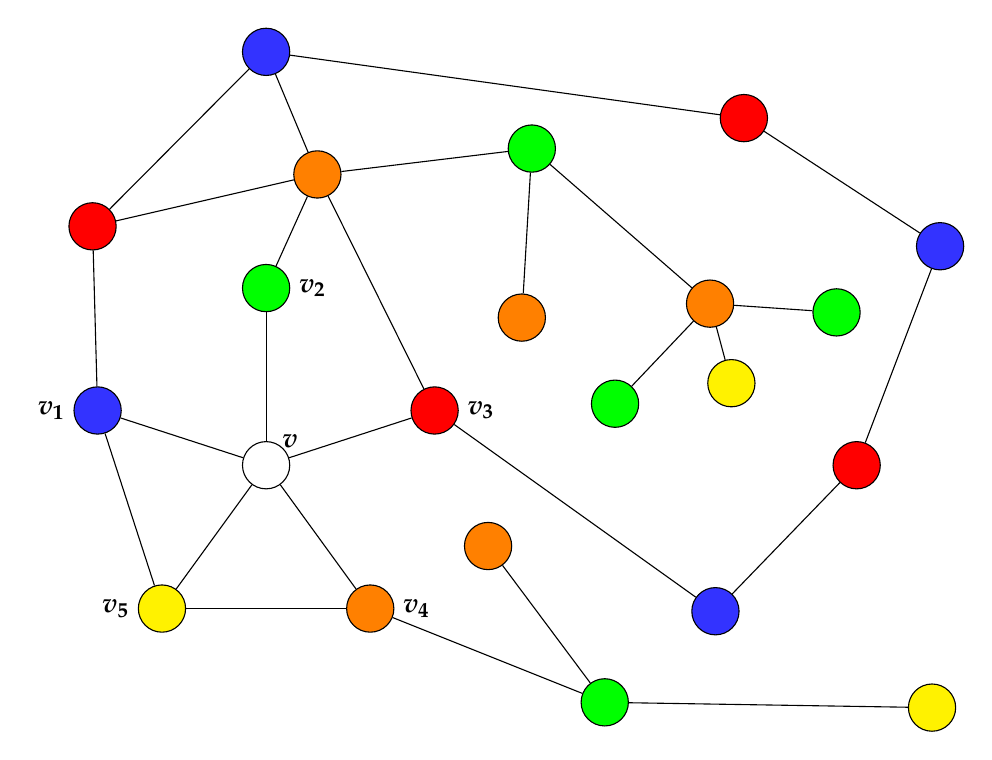
\begin{tikzpicture}[scale=.75,minimum size=6mm,inner sep=0pt]
\foreach \name/\color/\theta in
    {A/red/18,B/green/90,C/blue!80/162,D/yellow/234,E/orange/306}
  \node[circle,draw,fill=\color] (\name) at (\theta:3) {};
\node[circle,draw] (O) at (0,0) {};
\node[above right] at (O) {$\bm{v}$};

\node[right,xshift=8pt] at (A) {$\bm{v_3}$};
\node[right,xshift=8pt] at (B) {$\bm{v_2}$};
\node[left,,xshift=-8pt] at (C) {$\bm{v_1}$};
\node[left,,xshift=-8pt] at (D) {$\bm{v_5}$};
\node[right,xshift=8pt] at (E) {$\bm{v_4}$};

\foreach \name in {A,B,C,D,E}
  \draw (O) -- (\name);
  
\node[circle,draw,fill=red]  (X1) at (126:5) {};
\node[circle,draw,fill=blue!80] (X2) at (90:7)  {};
\node[circle,draw,fill=red]  (X3) at (36:10) {};
\node[circle,draw,fill=blue!80] (X4) at (18:12) {};
\node[circle,draw,fill=red]  (X5) at (0:10) {};
\node[circle,draw,fill=blue!80] (X6) at (-18:8) {};
\draw (C)  -- (X1);
\draw (X1) -- (X2);
\draw (X2) -- (X3);
\draw (X3) -- (X4);
\draw (X4) -- (X5);
\draw (X5) -- (X6);
\draw (X6) -- (A);

\node[circle,draw,fill=orange]  (Y1)  at (80:5) {};
\node[circle,draw,fill=green]   (Y2)  at (50:7)  {};
\node[circle,draw,fill=orange]  (Y3A) at (20:8) {};
\node[circle,draw,fill=orange]  (Y3B) at (30:5) {};
\node[circle,draw,fill=green]   (Y4A) at (10:6) {};
\node[circle,draw,fill=yellow]   (Y4B) at (10:8) {};
\node[circle,draw,fill=green]   (Y4C) at (15:10) {};
\node[circle,draw,fill=green]   (Y5)  at (-35:7) {};
\node[circle,draw,fill=yellow]  (Y6A) at (-20:12) {};
\node[circle,draw,fill=orange]  (Y6B) at (-20:4) {};
\draw (B)  -- (Y1);
\draw (Y1) -- (Y2);
\draw (Y2) -- (Y3A);
\draw (Y2) -- (Y3B);
\draw (Y3A) -- (Y4A);
\draw (Y3A) -- (Y4B);
\draw (Y3A) -- (Y4C);
\draw (E)  -- (Y5);
\draw (Y5) -- (Y6A);
\draw (Y5) -- (Y6B);
\draw (A) -- (Y1);
\draw (X2) -- (Y1);
\draw (X1) -- (Y1);
\draw (D) -- (E);
\draw (D) -- (C);
\end{tikzpicture}
\end{center}
Consider the vertex $v_1$ colored blue and the vertex $v_3$ colored red, and suppose that they are contained in a chain (with colors red and blue). By adding the vertex $v$ and the edges $\overline{vv_1},\overline{vv_3}$ to the chain we obtain a closed path $P$ (denoted in the diagram below by a double line) that divides the plane into an ``inside'' region and an ``outside'' region.
\begin{center}
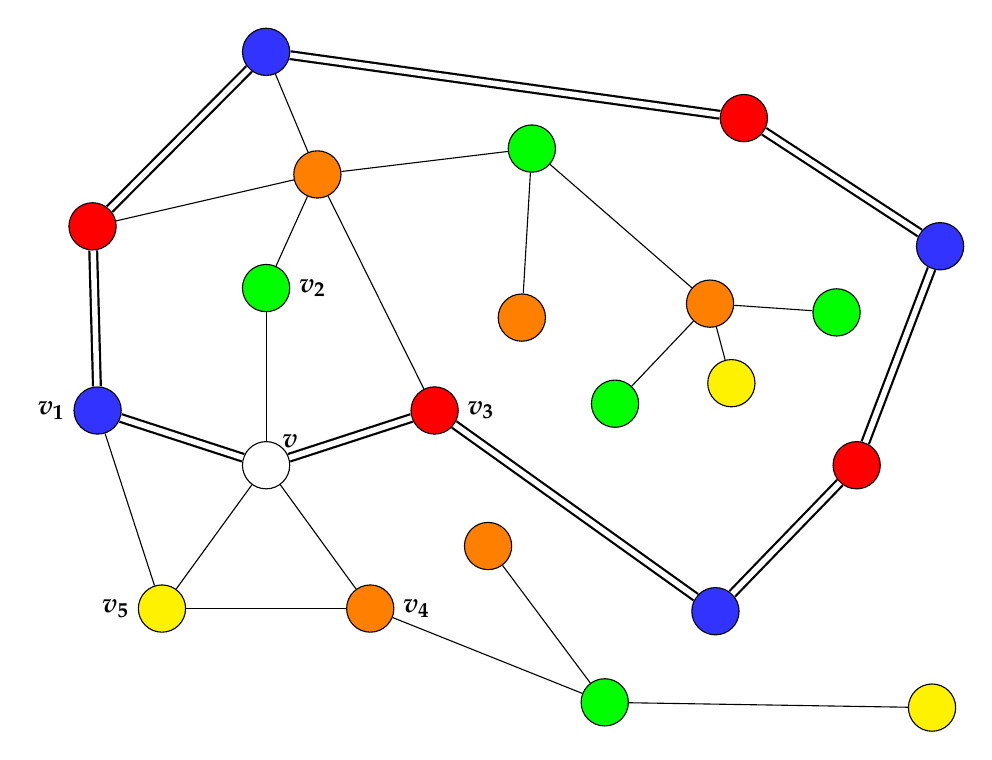
\begin{tikzpicture}[scale=.75,minimum size=6mm,inner sep=0pt]
\foreach \name/\color/\theta in
    {A/red/18,B/green/90,C/blue!80/162,D/yellow/234,E/orange/306}
  \node[circle,draw,fill=\color] (\name) at (\theta:3) {};
\node[circle,draw] (O) at (0,0) {};
\node[above right] at (O) {$\bm{v}$};

\node[right,xshift=8pt] at (A) {$\bm{v_3}$};
\node[right,xshift=8pt] at (B) {$\bm{v_2}$};
\node[left,,xshift=-8pt] at (C) {$\bm{v_1}$};
\node[left,,xshift=-8pt] at (D) {$\bm{v_5}$};
\node[right,xshift=8pt] at (E) {$\bm{v_4}$};

\foreach \name in {A,B,C,D,E}
  \draw (O) -- (\name);
  
\node[circle,draw,fill=red]  (X1) at (126:5) {};
\node[circle,draw,fill=blue!80] (X2) at (90:7)  {};
\node[circle,draw,fill=red]  (X3) at (36:10) {};
\node[circle,draw,fill=blue!80] (X4) at (18:12) {};
\node[circle,draw,fill=red]  (X5) at (0:10) {};
\node[circle,draw,fill=blue!80] (X6) at (-18:8) {};
\draw[thick,double distance=2pt] (C)  -- (X1);
\draw[thick,double distance=2pt] (X1) -- (X2);
\draw[thick,double distance=2pt] (X2) -- (X3);
\draw[thick,double distance=2pt] (X3) -- (X4);
\draw[thick,double distance=2pt] (X4) -- (X5);
\draw[thick,double distance=2pt] (X5) -- (X6);
\draw[thick,double distance=2pt] (X6) -- (A);
\draw[thick,double distance=2pt] (A) -- (O) -- (C);

\node[circle,draw,fill=orange]  (Y1)  at (80:5) {};
\node[circle,draw,fill=green]   (Y2)  at (50:7)  {};
\node[circle,draw,fill=orange]  (Y3A) at (20:8) {};
\node[circle,draw,fill=orange]  (Y3B) at (30:5) {};
\node[circle,draw,fill=green]   (Y4A) at (10:6) {};
\node[circle,draw,fill=yellow]   (Y4B) at (10:8) {};
\node[circle,draw,fill=green]   (Y4C) at (15:10) {};
\node[circle,draw,fill=green]   (Y5)  at (-35:7) {};
\node[circle,draw,fill=yellow]  (Y6A) at (-20:12) {};
\node[circle,draw,fill=orange]  (Y6B) at (-20:4) {};
\draw (B)  -- (Y1);
\draw (Y1) -- (Y2);
\draw (Y2) -- (Y3A);
\draw (Y2) -- (Y3B);
\draw (Y3A) -- (Y4A);
\draw (Y3A) -- (Y4B);
\draw (Y3A) -- (Y4C);
\draw (E)  -- (Y5);
\draw (Y5) -- (Y6A);
\draw (Y5) -- (Y6B);
\draw (A) -- (Y1);
\draw (X2) -- (Y1);
\draw (X1) -- (Y1);
\draw (D) -- (E);
\draw (D) -- (C);
\end{tikzpicture}
\end{center}
Consider the vertex $v_2$ colored green and the vertex $v_4$ colored orange. These vertices \emph{cannot} be contained in a single chain (with colors green and orange) because $v_2$ is \emph{inside} $P$ and $v_4$ is \emph{outside} $P$, so any path connecting them must cross $P$, contradicting the assumption that the graph is planar.\footnote{This follows from the \emph{Jordan curve theorem} which is intuitively obvious but very difficult to prove.} In the following diagram the two \emph{unconnected} chains which contain $v_2$ and $v_4$ are denoted with a double dashed line.
\begin{center}
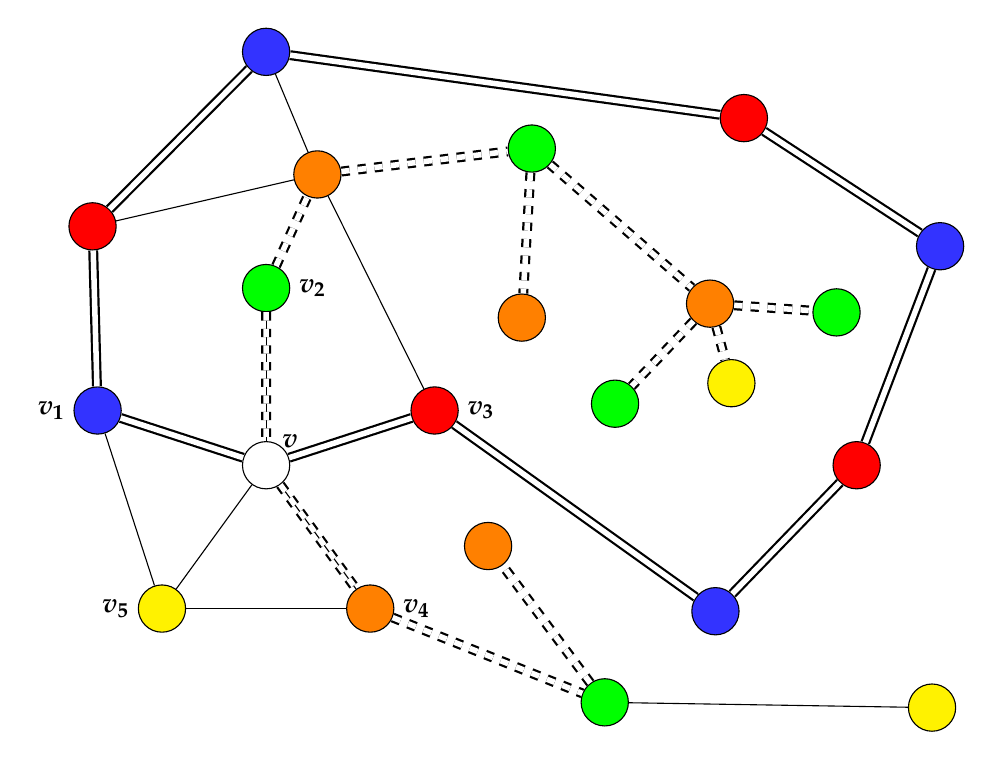
\begin{tikzpicture}[scale=.75,minimum size=6mm,inner sep=0pt]
\foreach \name/\color/\theta in
    {A/red/18,B/green/90,C/blue!80/162,D/yellow/234,E/orange/306}
  \node[circle,draw,fill=\color] (\name) at (\theta:3) {};
\node[circle,draw] (O) at (0,0) {};
\node[above right] at (O) {$\bm{v}$};

\node[right,xshift=8pt] at (A) {$\bm{v_3}$};
\node[right,xshift=8pt] at (B) {$\bm{v_2}$};
\node[left,,xshift=-8pt] at (C) {$\bm{v_1}$};
\node[left,,xshift=-8pt] at (D) {$\bm{v_5}$};
\node[right,xshift=8pt] at (E) {$\bm{v_4}$};

\foreach \name in {A,B,C,D,E}
  \draw (O) -- (\name);
  
\node[circle,draw,fill=red]  (X1) at (126:5) {};
\node[circle,draw,fill=blue!80] (X2) at (90:7)  {};
\node[circle,draw,fill=red]  (X3) at (36:10) {};
\node[circle,draw,fill=blue!80] (X4) at (18:12) {};
\node[circle,draw,fill=red]  (X5) at (0:10) {};
\node[circle,draw,fill=blue!80] (X6) at (-18:8) {};

\draw[thick,double distance=2pt] (C)  -- (X1);
\draw[thick,double distance=2pt] (X1) -- (X2);
\draw[thick,double distance=2pt] (X2) -- (X3);
\draw[thick,double distance=2pt] (X3) -- (X4);
\draw[thick,double distance=2pt] (X4) -- (X5);
\draw[thick,double distance=2pt] (X5) -- (X6);
\draw[thick,double distance=2pt] (X6) -- (A);
\draw[thick,double distance=2pt] (A) -- (O) -- (C);

\node[circle,draw,fill=orange]  (Y1)  at (80:5) {};
\node[circle,draw,fill=green]   (Y2)  at (50:7)  {};
\node[circle,draw,fill=orange]  (Y3A) at (20:8) {};
\node[circle,draw,fill=orange]  (Y3B) at (30:5) {};
\node[circle,draw,fill=green]   (Y4A) at (10:6) {};
\node[circle,draw,fill=yellow]   (Y4B) at (10:8) {};
\node[circle,draw,fill=green]   (Y4C) at (15:10) {};
\node[circle,draw,fill=green]   (Y5)  at (-35:7) {};
\node[circle,draw,fill=yellow]  (Y6A) at (-20:12) {};
\node[circle,draw,fill=orange]  (Y6B) at (-20:4) {};
\draw[thick,dashed,double distance=2pt] (B)  -- (O) -- (E);
\draw[thick,dashed,double distance=2pt] (B)  -- (Y1);
\draw[thick,dashed,double distance=2pt] (Y1) -- (Y2);
\draw[thick,dashed,double distance=2pt] (Y2) -- (Y3A);
\draw[thick,dashed,double distance=2pt] (Y2) -- (Y3B);
\draw[thick,dashed,double distance=2pt] (Y3A) -- (Y4A);
\draw[thick,dashed,double distance=2pt] (Y3A) -- (Y4B);
\draw[thick,dashed,double distance=2pt] (Y3A) -- (Y4C);
\draw[thick,dashed,double distance=2pt] (E)  -- (Y5);
\draw[thick,dashed,double distance=2pt] (Y5) -- (Y6B);
\draw (Y5) -- (Y6A);
\draw (A) -- (Y1);
\draw (X2) -- (Y1);
\draw (X1) -- (Y1);
\draw (D) -- (E);
\draw (D) -- (C);
\end{tikzpicture}
\end{center}
\newpage
We can exchange the colors on the chain containing  $v_2$, and this will not change the fact that $G'$ is five- colored. Since $v_2$ and $v_4$ are now both colored orange, $v$ can be colored green to obtain a five-coloring of $G$.\qed
\begin{center}
\begin{tikzpicture}[scale=.75,minimum size=6mm,inner sep=0pt]
\foreach \name/\color/\theta in
    {A/red/18,B/orange/90,C/blue!80/162,D/yellow/234,E/orange/306}
  \node[circle,draw,fill=\color] (\name) at (\theta:3) {};
\node[circle,draw,fill=green] (O) at (0,0) {};
\node[above right] at (O) {$\bm{v}$};

\node[right,xshift=8pt] at (A) {$\bm{v_3}$};
\node[right,xshift=8pt] at (B) {$\bm{v_2}$};
\node[left,,xshift=-8pt] at (C) {$\bm{v_1}$};
\node[left,,xshift=-8pt] at (D) {$\bm{v_5}$};
\node[right,xshift=8pt] at (E) {$\bm{v_4}$};

\foreach \name in {A,B,C,D,E}
  \draw (O) -- (\name);
  
\node[circle,draw,fill=red]  (X1) at (126:5) {};
\node[circle,draw,fill=blue!80] (X2) at (90:7)  {};
\node[circle,draw,fill=red]  (X3) at (36:10) {};
\node[circle,draw,fill=blue!80] (X4) at (18:12) {};
\node[circle,draw,fill=red]  (X5) at (0:10) {};
\node[circle,draw,fill=blue!80] (X6) at (-18:8) {};

\draw[thick,double distance=2pt] (C)  -- (X1);
\draw[thick,double distance=2pt] (X1) -- (X2);
\draw[thick,double distance=2pt] (X2) -- (X3);
\draw[thick,double distance=2pt] (X3) -- (X4);
\draw[thick,double distance=2pt] (X4) -- (X5);
\draw[thick,double distance=2pt] (X5) -- (X6);
\draw[thick,double distance=2pt] (X6) -- (A);
\draw[thick,double distance=2pt] (A) -- (O) -- (C);

\draw[thick,dashed,double distance=2pt] (B)  -- (O) -- (E);
\draw[thick,dashed,double distance=2pt] (B)  -- (Y1);
\draw[thick,dashed,double distance=2pt] (Y1) -- (Y2);
\draw[thick,dashed,double distance=2pt] (Y2) -- (Y3A);
\draw[thick,dashed,double distance=2pt] (Y2) -- (Y3B);
\draw[thick,dashed,double distance=2pt] (Y3A) -- (Y4A);
\draw[thick,dashed,double distance=2pt] (Y3A) -- (Y4B);
\draw[thick,dashed,double distance=2pt] (Y3A) -- (Y4C);
\draw[thick,dashed,double distance=2pt] (E)  -- (Y5);
\draw[thick,dashed,double distance=2pt] (Y5) -- (Y6B);

\node[circle,draw,fill=green]  (Y1)  at (80:5) {};
\node[circle,draw,fill=orange]   (Y2)  at (50:7)  {};
\node[circle,draw,fill=green]  (Y3A) at (20:8) {};
\node[circle,draw,fill=green]  (Y3B) at (30:5) {};
\node[circle,draw,fill=orange]   (Y4A) at (10:6) {};
\node[circle,draw,fill=yellow]   (Y4B) at (10:8) {};
\node[circle,draw,fill=orange]   (Y4C) at (15:10) {};
\node[circle,draw,fill=green]   (Y5)  at (-35:7) {};
\node[circle,draw,fill=yellow]  (Y6A) at (-20:12) {};
\node[circle,draw,fill=orange]  (Y6B) at (-20:4) {};


\draw (Y5) -- (Y6A);
\draw (A) -- (Y1);
\draw (X2) -- (Y1);
\draw (X1) -- (Y1);
\draw (D) -- (E);
\draw (D) -- (C);
\end{tikzpicture}
\end{center}

%%%%%%%%%%%%%%%%%%%%%%%%%%%%%%%%%%%%%%%%%%%%%%%%%%%%%%%%%%%
%%%%%%%%%%%%%%%%%%%%%%%%%%%%%%%%%%%%%%%%%%%%%%%%%%%%%%%%%%%
%%%%%%%%%%%%%%%%%%%%%%%%%%%%%%%%%%%%%%%%%%%%%%%%%%%%%%%%%%%
%%%%%%%%%%%%%%%%%%%%%%%%%%%%%%%%%%%%%%%%%%%%%%%%%%%%%%%%%%%


\section{Kempe's incorrect proof of the four-color theorem}\label{s.kempe}

The four-color theorem was posed and conjectured to hold in 1852. In 1879, Alfred B. Kempe published a proof of the theorem,  but eleven years later, in 1890, Percy J. Heawood found an error in the proof. Nevertheless, Kempe's work is important because: (1) it provided a correct proof of the five-color theorem, and (2) his proof contained the basic ideas that were used by Kenneth Appel and Wolfgang Haken in their correct proof published in 1976.

\textbf{Proof} The base case of the induction and most of the proof is the same as that of the five-color theorem. The new case that must be considered is a vertex $v$ with five neighbors which, by the inductive hypothesis, are colored with four colors after removing $v$.

In the left diagram below, there are two vertices $v_2,v_5$ colored blue. Consider the blue-green chain containing $v_2$ and the blue-yellow chain containing $v_5$. The blue-green chain is contained within the closed path defined by the red-yellow chain containing $v_1,v_3$ and the blue-yellow chain in contained within the closed path defined by the red-green chain containing $v_1,v_4$.

Now exchange the colors on the blue-green chain and on the blue-yellow chain (right diagram below). The result is that the neighbors of $v$ are colored with the three colors red, green and yellow, leaving blue free to color $v$.

\begin{center}
\begin{tikzpicture}[scale=.6,minimum size=6mm,inner sep=0pt]

% Draw center node and adjacent nodes
\foreach \name/\color/\theta in
    {A/yellow/18,B/blue!80/90,C/red/162,D/blue!80/234,E/green/306}
  \node[circle,draw,fill=\color] (\name) at (\theta:3) {};
\node[circle,draw] (O) at (0,0) {};
\node[above right]     at (O) {$\bm{v}$};

\node[right,xshift=10pt] at (A) {$\bm{v_3}$};
\node[left,xshift=-8pt]  at (B) {$\bm{v_2}$};
\node[left,xshift=-8pt]  at (C) {$\bm{v_1}$};
\node[left,xshift=-8pt]  at (D) {$\bm{v_5}$};
\node[right,xshift=8pt]  at (E) {$\bm{v_4}$};

% Draw red-yellow path
\node[circle,draw,fill=yellow]  (X1) at (126:5) {};
\node[circle,draw,fill=red] (X2) at (45:8)  {};

\draw[thick,double distance=2pt] 
  (C) -- (X1) -- (X2) -- (A) -- (O);
\draw[thick,double distance=6pt] (O) -- (C);

% Draw blue-green nodes within red-yellow path
\node[circle,draw,fill=green] (Y1)  at (50:5) {};

% Draw red-green path
\node[circle,draw,fill=green] (Z1)  at (-160:5) {};
\node[circle,draw,fill=red]   (Z2)  at (-80:6)  {};

%\draw[thick,dashed,double distance=6pt] (O) -- (C);
\draw[thick,dashed,double distance=2pt] 
  (O) -- (C) -- (Z1) -- (Z2) -- (E) -- (O);

% Draw blue-yellow nodes within red-green path
\node[circle,draw,fill=yellow]   (U1)  at (-90:4)  {};

% Connect adjacent nodes not in paths
\draw (X1) -- (B) -- (Y1) -- (A) -- (B) -- 
      (C) -- (D) -- (E) -- (A);
\draw (Z2) -- (U1) -- (D) -- (O) -- (B);

%\end{tikzpicture}
%\end{center}

\begin{scope}[xshift=12cm]
%\begin{center}
%\begin{tikzpicture}[scale=.6,minimum size=6mm,inner sep=0pt]

% Draw center node and adjacent nodes
\foreach \name/\color/\theta in
    {A/yellow/18,B/green/90,C/red/162,D/yellow/234,E/green/306}
  \node[circle,draw,fill=\color] (\name) at (\theta:3) {};
\node[circle,draw,fill=blue!80] (O) at (0,0) {};
\node[above right]     at (O) {$\bm{v}$};

\node[right,xshift=10pt] at (A) {$\bm{v_3}$};
\node[left,xshift=-8pt]  at (B) {$\bm{v_2}$};
\node[left,xshift=-8pt]  at (C) {$\bm{v_1}$};
\node[left,xshift=-8pt]  at (D) {$\bm{v_5}$};
\node[right,xshift=8pt]  at (E) {$\bm{v_4}$};

% Draw red-yellow path
\node[circle,draw,fill=yellow]  (X1) at (126:5) {};
\node[circle,draw,fill=red] (X2) at (45:8)  {};

\draw[thick,double distance=2pt] 
  (C) -- (X1) -- (X2) -- (A) -- (O);
\draw[thick,double distance=6pt] (O) -- (C);

% Draw blue-green nodes within red-yellow path
\node[circle,draw,fill=blue!80] (Y1)  at (50:5) {};

% Draw red-green path
\node[circle,draw,fill=green] (Z1)  at (-160:5) {};
\node[circle,draw,fill=red]   (Z2)  at (-80:6)  {};

\draw[thick,dashed,double distance=2pt] 
  (O) -- (C) -- (Z1) -- (Z2) -- (E) -- (O);

% Draw blue-yellow nodes within red-green path
\node[circle,draw,fill=blue!80]   (U1)  at (-90:4)  {};

% Connect adjacent nodes not in paths
\draw (X1) -- (B) -- (Y1) -- (A) -- (B) -- 
      (C) -- (D) -- (E) -- (A);
\draw (Z2) -- (U1) -- (D) -- (O) -- (B);
\end{scope}
\end{tikzpicture}
\end{center}

Heawood noted that the closed paths defined by the red-yellow and red-green chains can share red vertices ($v_1$ and the red vertex below $v_4$ in the left diagram below).
When the colors are exchanged in the blue-green and blue-yellow chains, it is possible for blue vertices to be connected (right diagram below), so the coloring is no longer correct.

\begin{center}
\begin{tikzpicture}[scale=.6,minimum size=6mm,inner sep=0pt]

% Draw center node and adjacent nodes
\foreach \name/\color/\theta in
    {A/yellow/18,B/blue!80/90,C/red/162,D/blue!80/234,E/green/306}
  \node[circle,draw,fill=\color] (\name) at (\theta:3) {};
\node[circle,draw] (O) at (0,0) {};
\node[above right]     at (O) {$\bm{v}$};

\node[right,xshift=10pt] at (A) {$\bm{v_3}$};
\node[right,xshift=8pt]  at (B) {$\bm{v_2}$};
\node[above right,xshift=8pt]  at (C) {$\bm{v_1}$};
\node[below right,yshift=-8pt] at (D) {$\bm{v_5}$};
\node[right,xshift=8pt]  at (E) {$\bm{v_4}$};

% Draw red-yellow path
\node[circle,draw,fill=yellow] (X1) at (-170:5) {};
\node[circle,draw,fill=red]    (X2) at (-80:7)  {};

\draw[thick,double distance=2pt] (A) -- (O);
\draw[thick,double distance=6pt] (O) -- (C);
\draw[thick,double distance=2pt] (C) --(X1) -- (X2);
\draw[thick,double distance=2pt,bend right=40] (X2) to (A);

% Draw red-green path
\node[circle,draw,fill=green] (Y1) at (100:6)  {};

\draw[dashed,thick,double distance=2pt] (O) -- (C) -- (Y1);
\draw[dashed,thick,double distance=2pt] 
  (Y1) .. controls (40:10) and (-50:9) .. (X2);
\draw[dashed,thick,double distance=2pt] (X2) -- (E) -- (O);

% Draw adjacent nodes
\draw (X1) -- (D) -- (O) -- (B) -- (Y1) -- (X1);

%\end{tikzpicture}
%\end{center}

\begin{scope}[xshift=12cm]
%\begin{center}
%\begin{tikzpicture}[scale=.6,minimum size=6mm,inner sep=0pt]

% Draw center node and adjacent nodes
\foreach \name/\color/\theta in
    {A/yellow/18,B/green/90,C/red/162,D/yellow/234,E/green/306}
  \node[circle,draw,fill=\color] (\name) at (\theta:3) {};
\node[circle,draw,fill=blue!80] (O) at (0,0) {};
\node[above right]     at (O) {$\bm{v}$};

\node[right,xshift=10pt] at (A) {$\bm{v_3}$};
\node[right,xshift=8pt]  at (B) {$\bm{v_2}$};
\node[above right,xshift=8pt]  at (C) {$\bm{v_1}$};
\node[below right,yshift=-8pt] at (D) {$\bm{v_5}$};
\node[right,xshift=8pt]  at (E) {$\bm{v_4}$};


% Draw red-yellow path
\node[circle,draw,fill=blue!80] (X1) at (-170:5) {};
\node[circle,draw,fill=red]  (X2) at (-80:7)  {};

\draw[thick,double distance=2pt] (A) -- (O);
\draw[thick,double distance=6pt] (O) -- (C);
\draw[thick,double distance=2pt] (C) --(X1) -- (X2);
\draw[thick,double distance=2pt,bend right=40] (X2) to (A);

% Draw red-green path
\node[circle,draw,fill=blue!80] (Y1) at (100:6)  {};

\draw[dashed,thick,double distance=2pt] (O) -- (C) -- (Y1);
\draw[dashed,thick,double distance=2pt] 
  (Y1) .. controls (40:10) and (-50:9) .. (X2);
\draw[dashed,thick,double distance=2pt] (X2) -- (E) -- (O);

% Draw adjacent nodes
\draw (X1) -- (D) -- (O) -- (B) -- (Y1) -- (X1);
\end{scope}
\end{tikzpicture}
\end{center}

\newpage

\nocite{*}
\bibliographystyle{plain}
\bibliography{five-en}
\end{document}
